
\documentclass[final]{scrartcl}

\usepackage[
  bibresource=../references.bib,
  bibstyle=alphabetic,
]{preamble-summary}


\title{Context Reasoning for Role-Based Models}
\author{Stephan Böhme}
\date{Summary}

\begin{document}

\maketitle

\noindent
Nowadays, we are literally everywhere surrounded by software systems. Current developments indicate
a continuing growth in the future.  Not only the amount of systems increases, but also the
requirements and expectations users impose on current software steadily rise. Modern software
systems should cope with very complex scenarios. This includes the ability of context-awareness and
self-adaptability. For example, a robot in a smart factory should recognize when a human co-worker
approaches and switch to a different, human-friendly working mode accordingly. Similarly, software
in autonomous cars or in the area of smart homes needs to adapt to various situations of which some
are not even stated explicitly.
%
Furthermore, software must be easily maintainable and, when necessary, changes on the system should
be realised without much down time which, for example, in a smart factory is very costly.

%%%

In order to achieve all these goals, the concept of \emph{roles} is very promising. First introduced
by Bachman~\cite{BaD-VLDB77}, roles appeared over the last decades in several fields of computer
science. Most prominent is the \emph{role-based access
  control}~\cite{FeKC-RBAC03,AlFe-ECS11,SaCF-IEEE96}, albeit it is only a special application for
roles with a narrow scope. Roles are also introduced, for example, in data
modelling~\cite{Ha-ORM2006}, conceptual modelling~\cite{Stei-DKE00,Gui-PHD05,Stei-AO07} and
programming languages~\cite{BaBT-SAC06,Herr-AO07,BaGE-ECOOP07}.

The relational or context-dependent properties and behaviour of objects are transferred into the
roles that an object plays in a certain context. This paradigm also supports Dijkstra's separation of
concerns~\cite{Dij-SelWrCom82} which simplifies development and maintenance of such systems.  Due to
the use of roles, \emph{role-based systems} can model application domains cleaner and more
structured, since ontologically different entities are modelled by different concepts.

Let us consider, for example, the concepts of $\mathsf{Person}$ and $\mathsf{Customer}$. With an
object-oriented approach of inheritance as a specialization relation, we could model
$\mathsf{Customer}$ as a subclass of $\mathsf{Person}$, as not every person is a customer.
On the other hand, if we restrict our domain to a business context and add the concept of a
$\mathsf{Company}$, the inheritance relation would flip and we also have $\mathsf{Company}$ as
subclass of $\mathsf{Customer}$.  This conflict can be resolved by recognising
$\mathsf{Person}$ and $\mathsf{Company}$ as context-independent basic concepts, so-called
\emph{natural types} and $\mathsf{Customer}$ as a role a person or company can play in a
business context. Here, it also becomes apparent that the concept of a \emph{context} is closely
related to a role.

While role-based modelling provides the means to handle and model complex and context-dependent
domains in a well-structured and modular way, the process can still be tedious, hard and
error-prone. Due to the sophisticated semantics of roles, contexts and many different kinds of
constraints, unintended implications or even inconsistencies can easily be hidden within such a
model. Since it is nearly impossible to uncover all inferences, it becomes imperative for domain
analysts to reason on role-based models to find such implicit knowledge.  Here, a formally defined
role modelling language and a feasible logical formalism are required.

%%%%%%%%%%%%%%%%%%%%%%%%%%%%%%
% CROM
%%%%%%%%%%%%%%%%%%%%%%%%%%%%%%

In this thesis we focus on the \emph{Compartment Role Object Model (CROM)} \cite{KBG-SLE15} to model
dynamic, context-dependent domains. It introduces so-called \emph{compartment types} to represent
objectified contexts. These contain a set of \emph{role types}, i.e.\ the roles that can be played
in that context, a \emph{fills}-relation that constrains which natural types are allowed to play
certain role types, and a set of \emph{relationship types}, i.e.\ a set of binary relations.
%
\begin{figure}
  \centering
  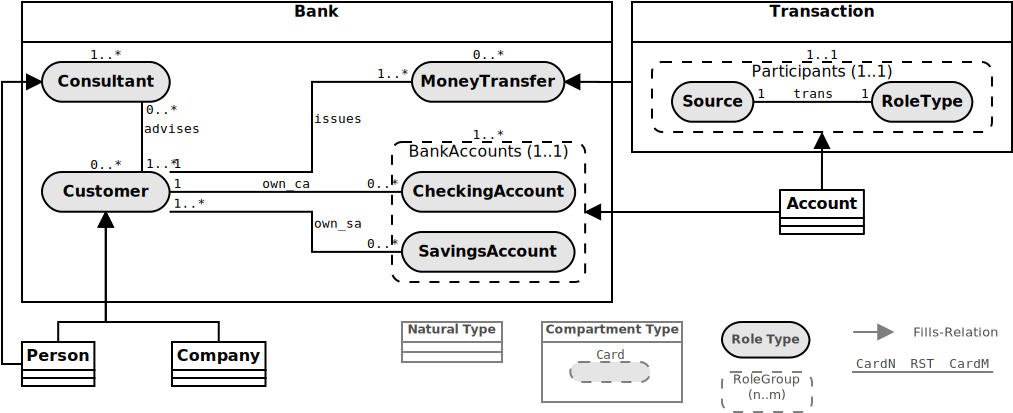
\includegraphics[width=\textwidth]{Bank-full-constraints}
  \caption{A bank example in CROM graphical notation}
  \label{fig:crom}
\end{figure}
%
Due to brevity we omit here the precise definitions of CROM and rather explain its expressiveness
with the help of an example. Figure~\ref{fig:crom} shows a small banking example. In the context of
a $\mathsf{Bank}$ there are the natural types $\mathsf{Person}$ and $\mathsf{Company}$ which can
``play'' the role of a $\mathsf{Customer}$ while only $\mathsf{Person}$s can be
$\mathsf{Consultant}$s. Additionally $\mathsf{Account}$s can be either $\mathsf{CheckingAccount}$s
or $\mathsf{SavingsAccounts}$ which in return can be $\mathsf{own}$ed by a customer. Furthermore, an
$\mathsf{Account}$ can be either the $\mathsf{Source}$ or the $\mathsf{Target}$ in the context of a
$\mathsf{Transaction}$. Then, this transaction can be a $\mathsf{MoneyTransfer}$ that is
$\mathsf{issue}$d by a $\mathsf{Customer}$ in the context of a $\mathsf{Bank}$. This illustrates
that compartments can again play roles within other compartments. At last, further constraints can
be imposed on the model. These include, among others, \emph{occurrence constraints} which restrict
the number of roles played within a compartment, i.e. a $\mathsf{Bank}$ has at least one
$\mathsf{Consultant}$, and \emph{cardinality constraints} which restrict the cardinalities of
relationship types, i.e. a $\mathsf{CheckingsAccount}$ is owned by exactly one $\mathsf{Customer}$.

However, reasoning directly on CROM models is not recommended as no elaborate reasoning algorithms
exist and due to the lack of tool support.  Therefore, we translate CROMs into a feasible logical
formalism which allows for efficient reasoning.

%%%%%%%%%%%%%%%%%%%%%%%%%%%%%%
% DLs
%%%%%%%%%%%%%%%%%%%%%%%%%%%%%%

As logical formalism we start with Description Logics (DLs) \cite{DLhandbook-07}. DLs are a
well-known formalism for knowledge representation. They possess formal semantics and allow to define
a variety of reasoning problems.
%
The basic building blocks in description logics are so-called \emph{concept names} and \emph{role
  names}. Concept names denote sets of domain elements. For example, the concept names
$\mathsf{Person}$ or $\mathsf{Bank}$ denote the sets of all persons or banks in a domain. Relational
structures are represented by so-called DL \emph{role names}, which are essentially binary relations
on the domain. The term ``role'' originates from the early knowledge representation system
KL-ONE~\cite{WoS-CMA133} and has only little in common with roles of role-based systems except that
it reflects the relational property of a role. A person which is related to a bank via a DL role
$\mathsf{customer}$ could be seen as someone playing the role of a customer in the context of a
bank. Besides that, DL roles are merely binary relations. With the help of \emph{concept} and
\emph{role constructors}, complex concepts and roles can be defined.  Which constructors are allowed
depends on the specific DL. Complex concepts can be used as descriptions and to classify domain
elements, e.g.\ the complex concept
\begin{align}
  \label{eq:1-1}
  \mathsf{NFL\_Player} \sqcap \mathsf{Healthy} \sqcap \exists.\mathsf{wins}(\mathsf{NFL\_Game})
\end{align}
describes the set of all healthy NFL players who win NFL games.

With the help of concepts, we can express our knowledge about a domain through \emph{DL
  axioms}. General knowledge is phrased via \emph{general concept inclusions (GCIs)}, which state
that one concept is a sub-concept of another. For example the GCI
\begin{align}
  \label{eq:1-2}
  \mathsf{NFL\_Player} \sqcap \mathsf{Healthy} \sqcap
  \exists.\mathsf{wins}(\mathsf{NFL\_Game}) \sqsubseteq \mathsf{Happy\_NFL\_Player}
\end{align}
states that a healthy NFL player who wins NFL games is a happy NFL player. Conversely, it does not say
anything on whether every happy NFL player is healthy or wins games. Facts about a domain can be
expressed via \emph{concept} and \emph{role assertions}.  To express facts, we also introduce
\emph{individual names} which denote single domain elements. As an example consider the following axioms:
\begin{gather}
  (\mathsf{NFL\_Player} \sqcap \mathsf{Healthy})(\text{\textit{AaronRodgers}})\label{eq:1-3}\\
  \mathsf{NFL\_Game}(\text{\textit{SuperBowlXLV}}),\label{eq:1-4}\\
  \mathsf{\mathsf{wins}}(\text{\textit{AaronRodgers}},\text{\textit{SuperBowlXLV}})\label{eq:1-5}
\end{gather}
The first two concept assertions~\eqref{eq:1-3} and~\eqref{eq:1-4} state that Aaron Rodgers is a healthy NFL player and that Super Bowl~XLV is
an NFL game, while~\eqref{eq:1-5} expresses that he won Super Bowl~XLV. So he is also a happy
NFL player, even if not stated explicitly.  A \emph{DL knowledge base} is a set of such axioms.

The semantics of DLs are defined in a model-theoretic way and capture exactly the above mentioned
intentions.  An interpretation~\I consists of a domain and an interpretation function~$\cdot^{\I}$
which maps concept, role and individual names, respectively, to subsets, binary relations and elements of the
domain.  From there, it is exactly defined how complex concepts must be
interpreted. For example, $(A\sqcap B)^{\I}$ is the intersection of $A^{\I}$ and $B^{\I}$.  The
concept name $\mathsf{NFL\_Player}$ itself has no meaning and an interpretation must make sure that
$\mathsf{NFL\_Player}^{\I}$ actually is the set of all NFL players.

Now, the most interesting reasoning problems are the \emph{consistency problem} and the \emph{entailment
problem}. A knowledge base is consistent if there exists some interpretation that \emph{models} the
knowledge base, i.e.\ an interpretation that fulfils all the axioms. An axiom is \emph{entailed} by
a knowledge base if every model of the knowledge base also models that axiom. For example, the following axiom is
entailed by~\eqref{eq:1-2} to~\eqref{eq:1-5}:
\begin{gather}
  \mathsf{Happy\_NFL\_Player}(\text{\textit{AaronRodgers}}).\label{eq:1-6}
\end{gather}


\begin{figure}
  \centering
  \begin{tikzpicture}
    \node[node, label={[align=right]180:\textsf{AaronRodgers},\\ $\mathsf{Healthy}$,\\
      $\mathsf{NFL\_Player}$,\\$\mathsf{Happy\_NFL\_Player}$}] (ar) at(-2,0) {}; 
    \node[node, label={[align=left]0:\textsf{SuperBowlXLV},\\ $\mathsf{NFL\_Game}$}] (sb45) at (2,0)
    {};
    \draw[edge] (ar) to[bend left=10] node{$\mathsf{wins}$} (sb45);
  \end{tikzpicture}
  \caption{Interpretation that models axioms~\eqref{eq:1-2} to~\eqref{eq:1-6}.}
  \label{fig:dl-example-intro}
\end{figure}

\noindent
Figure~\ref{fig:dl-example-intro} depicts an interpretation which is a model of axioms~\eqref{eq:1-2} to~\eqref{eq:1-6}.

%%%%%%%%%%%%%%%%%%%%%%%%%%%%%%
% conDLs
%%%%%%%%%%%%%%%%%%%%%%%%%%%%%%

However, classical DLs lack expressive power to formalise that some individuals satisfy certain
concepts and relate to other individuals depending on a \emph{specific context} which is needed to
reason on role-based systems.

To overcome that deficiency in expressiveness of classical DLs, often two-dimensional DLs are
employed~\cite{KG-JELIA10,KLGu-DL-11,KlGu-AAAI11,KG16}. This approach uses one DL \LM as the
\emph{meta logic} to represent the contexts and their relationships to each other, and combines it
with the \emph{object logic} \LO that captures the relational structure within each context.
%
Moreover, while some pieces of information depend on the context, e.g.\ the roles played by an
object within a compartment, other pieces of information are
shared throughout all contexts, e.g.\ the name or the age of a person typically stays the same
independent of the actual context.  Expressing this context-independent information requires that
some concepts and roles are designated to be \emph{rigid}, i.e.~they are required to be interpreted
the same in all contexts.  Unfortunately, if rigid roles are admitted, reasoning in the above
mentioned two-dimensional DLs of context turns out to be undecidable; see~\cite{KG-JELIA10}.

We propose and investigate a family of two-dimensional context DLs \LMLO that
meets the above requirements, but is a restricted form of the ones defined in~\cite{KG-JELIA10} in
the sense that we limit the interaction of \LM and \LO.  More precisely, in our family of
context DLs the meta logic can refer to the internal structure of each context, but not vice versa.
That means that information is viewed in a top-down manner, i.e.~information of different contexts
is strictly capsuled and can only be accessed from the meta level.  Hence, we cannot
express, for instance, that everybody who is employed by a company has a certain property in the
context of private life.  We show that reasoning in \LMLO stays decidable with
such a restriction, even in the presence of rigid roles.
%
In some sense this restriction is similar to what is done in~\cite{BaGL-KR08,BaGL-ToCL12,Lip-PhD14}
to obtain a decidable temporalised DL with rigid roles.  

\tableSyntaxSemanticsLMLO

The syntax and semantics of the object logic \LO are defined in the standard way. See the upper part
of Table~\ref{tab:syntax-semantics-dls} for the case where \LO is \SHOIQ.
%
The syntax of the meta logic \LM is enriched by the additional concept constructor of
\emph{referring concepts} which considers object axioms that would occur in a TBox or ABox, i.e.\
GCIs, concept and role assertions, as meta concepts (lower part of
Table~\ref{tab:syntax-semantics-dls}). An \emph{\LMLO-Boolean knowledge base (BKB)} consists of a
Boolean combination \Bmc of meta TBox and ABox axioms, a set \RO of object role axioms and a set \RM
of meta role axioms.
%
The semantics of \LMLO are defined by \emph{nested interpretations}. A nested interpretation \JJ
consists of a set \Cbb of \emph{contexts} (or possible worlds), an interpretation function
$\cdot^{\J}$ for the meta dimension, an object domain $\Delta^{\J}$ and a set of interpretation
functions $(\cdot^{\I_{c}})_{c\in\Cbb}$ for the object dimension. The interpretation functions and
the entailment relation $\models$ are defined in the standard way and they are extended to complex
concepts as shown in the right column of Table~\ref{tab:syntax-semantics-dls}. An \LMLO-BKB is
called \emph{consistent} if there exists a nested interpretation \J such that \J models \Bmc, \RM
and \RO. The \emph{consistency problem} in \LMLO is the problem of deciding whether a given
\LMLO-BKB is consistent.

To provide a better intuition on how our formalism works, we examine the following example.
Consider the following axioms:
\begin{align}
  \top & \sqsubseteq \oax{\exists\mathsf{worksFor}.\{\text{\textit{Siemens}}\} \sqsubseteq \exists\mathsf{hasAccessRights}.\{\text{\textit{Siemens}}\}}\label{eq:1-7} \\
  \mathsf{Work} & \sqsubseteq \oax{\mathsf{worksFor}(\text{\textit{Bob}},\text{\textit{Siemens}})} \label{eq:1-8}\\
  \oax{(\exists\mathsf{worksFor}.\top)(\text{\textit{Bob}})}\
  & \sqsubseteq\ \exists\mathsf{related}.(\mathsf{Private} \sqcap \oax{\mathsf{HasMoney}(\text{\textit{Bob}})})\label{eq:1-9} \\
  \top\
  & \sqsubseteq\ \oax{\exists\mathsf{isCustomerOf}.\top \sqsubseteq\mathsf{HasMoney}} \label{eq:1-10}\\
  \mathsf{Private}\
  & \sqsubseteq\ \oax{\mathsf{isCustomerOf}(\text{\textit{Bob}},\text{\textit{Siemens}})}\label{eq:1-11}\\
  \mathsf{Private} \sqcap \mathsf{Work}\
  & \sqsubseteq\ \bot\label{eq:1-12}\\
  \lnot \mathsf{Work}\
  & \sqsubseteq\ \oax{\exists\mathsf{worksFor}.\top\sqsubseteq\bot}\label{eq:1-13}
\end{align}
%
The first axiom states that in all contexts somebody who works for Siemens also has access rights to
certain data.  The second axiom states that Bob is an employee of Siemens in any work context.
Furthermore, Axioms~\eqref{eq:1-9} and~\eqref{eq:1-10} say intuitively that if Bob has a job, he
will earn money, which he can spend as a customer.  Axiom~\eqref{eq:1-11} formalises that Bob is a
customer of Siemens in any private context.  Moreover, Axiom~\eqref{eq:1-12} ensures that the
private contexts are disjoint from the work contexts.  Finally, Axiom~\eqref{eq:1-13} states that
the $\mathsf{worksFor}$ relation only exists in work
contexts. Figure~\ref{fig:example-interpretation} depicts a model of Axioms
\eqref{eq:1-7}~--~\eqref{eq:1-13}.

\begin{figure}[t]
  \centering
  \begin{tikzpicture}[auto]
    %\draw[thin,gray] (0,-2) grid (15,3);
    \node[rectangle,
          draw,
          rounded corners= 5mm, 
          %minimum height = 4cm, 
          %minimum width = 6cm,
          label={120:$\mathsf{Work}$}] (a) at (3.5,0){
            \begin{tikzpicture}
              \node[node,label={[align=right]180:\textit{Bob},\\ $\mathsf{Person}$}] (bob) at (0,3){};
              \node[node,label={60:$\mathsf{SSN}$}] (ssn) at (3.7,3){};
              \draw[edge] (bob) to[bend left=10] node{$\mathsf{hasSSN}$} (ssn);
              \node[node,label={[align=right]180:\textit{Siemens},\\ $\mathsf{Company}$}] (siem) at (1,0.5){};
              \draw[edge] (bob) to[bend right=15] node[mylabel,swap]{$\mathsf{worksFor}$} (siem);
              \draw[edge] (bob) to[bend left=15] node[mylabel]{$\mathsf{hasAccessRights}$} (siem);
              \node[node,label={[align=right]north east:$\mathsf{Person}$}] (ceo) at (3.2,0.5){};
              \draw[edge] (siem) to[bend left=10] node{$\mathsf{hasCEO}$} (ceo);
              \node at (1.8,0.2){$\ddots$};
            \end{tikzpicture}
          };
    \node[rectangle,
          draw,
          rounded corners= 5mm,
          %minimum height = 4cm,
          %minimum width = 6cm,
          label={120:$\mathsf{Private}$}] (b) at (11.0,0){
            \begin{tikzpicture}
              \node[node,label={[align=right]180:\textit{Bob},\\ $\mathsf{Person}$,\\ $\mathsf{HasMoney}$}] (bob) at (0,3){};
              \node[node,label={60:$\mathsf{SSN}$}] (ssn) at (3,3){};
              \draw[edge] (bob) to[bend left=10] node{$\mathsf{hasSSN}$} (ssn);
            \node[node,label={[align=right]180:\textit{Siemens},\\ $\mathsf{Company}$}] (siem) at (1,0.5){};
              \draw[edge] (bob) to[bend left=15] node[mylabel]{$\mathsf{isCustomerOf}$} (siem);
              \node[node,label={[align=right]north east:$\mathsf{Person}$}] (ceo) at (2.5,0.5){};
            \end{tikzpicture}
          };
    \draw[edge] (a.east) to[bend left] node{$\mathsf{related}$} (b.west);
  \end{tikzpicture}
  \caption{Nested interpretation that models of Axioms \eqref{eq:1-7}--~\eqref{eq:1-13}}
  \label{fig:example-interpretation}
\end{figure}

As a basis for any further application of a newly defined logical framework a thorough analysis of
the computational complexities is necessary. We focus in this thesis on the complexity of the
consistency problem in \LMLO. The results are shown in Table~\ref{tab:compl-results}
In this summary we only want to sketch the ideas how to obtain the upper bounds, since the main
lemma is reused for the implementation of the reasoner later.

We proceed similar to what was done for \ALC-LTL in \cite{BaGL-KR08,BaGL-ToCL12} and reduce the
consistency problem to two separate decision problems. For the first decision problem, we consider
the so-called \emph{outer abstraction}, which is the \LM knowledge base obtained by replacing each
referring m-concept of the form \oalpha by a fresh concept name such that there is a 1--1
relationship between them.

This outer abstraction does not only need to be consistent, it must be consistent in the sense that
only certain sets of object axioms hold in each context. This additional request is defined by the
\emph{outer consistency w.r.t~\Xmc}. Furthermore, the second decision problem that we use for deciding consistency is needed to make sure that such a
set of abstracted concept names is admissible in the following sense.
\begin{definition}[Admissibility]\label{def:admissibility}
  Let $\Xmc=\{X_1,~\dots,\ X_k\}\subseteq\powerset{\ran(\bsf)}$.  We call \Xmc \emph{admissible} if
  there exist \Osig-interpretations $\I_1=(\Delta,\cdot^{\I_1})$,~\dots,
  $\I_k=(\Delta,\cdot^{\I_k})$ such that
  \begin{itemize}
  \item $x^{\I_i}=x^{\I_j}$ for all $x\in\OI\cup\OCR\cup\ORR$ and all $i,j\in\{1,\dots,k\}$, and
  \item every $\I_i$, $1\le i\le k$, is a model of the \LO-BKB $\Bmf_{X_{i}}= (\B_{X_i},\RO)$
    over~\Osig where
    \begin{align*}
      \B_{X_i}&\coloneqq\bigwedge_{\bsf(\oalpha)\in X_i}\alpha\ \land
      \bigwedge_{\bsf(\oalpha)\in\ran(\bsf)\setminus X_i}\lnot\alpha.
    \end{align*}
  \end{itemize}
  \vspace{-1.7\baselineskip}
\end{definition}

Now, the main lemma in this section states that the consistency problem in \LMLO can be reduced into
two separate decision problems.

\begin{lemma}\label{lem:admissible-and-outerConsistent}%
  The \LMLO-BKB~\Bmc is consistent iff there is a set
  $\Xmc\subseteq\powerset{\ran(\bsf)}$ such that
  \begin{enumerate}
  \item \Xmc is admissible, and
  \item the outer abstraction of \Bmc is outer consistent w.r.t.~\Xmc.
  \end{enumerate}
\end{lemma}

Based on this lemma, we can distinguish the three settings whether rigid concepts or rigid roles are
admitted in the BKB. Depending on these settings and on which DL is used as object or meta logic,
several complexity results were obtained and are summarized in Table~\ref{tab:compl-results}.

\TableComplexityResults




%%%%%%%%%%%%%%%%%%%%%%%%%%%%%%
% Mapping
%%%%%%%%%%%%%%%%%%%%%%%%%%%%%%



Besides the capability of context description logics to formalise role-based models, it is rather
hard for domain analysts---who in general are not experts in DLs---to grasp the precise semantics of
the ontology, and to define the contextualised ontology in a way that all entities and constraints
appearing in the role-based model are mapped correctly. Therefore, it would be ideal to have an
algorithm that translates role-based models into context DL knowledge bases.  In this thesis, we
present exactly such a mapping.

We already decided for CROM as a modelling language due to its formal semantics. This is important
since otherwise we cannot ensure that the intended meaning of every
model is correctly translated into the ontology. 

There is also some freedom on how to express roles and role-playing in an ontology. While it is
important to consider the ontological nature of roles such as identity or rigidity, we also have to
consider practical reasons. Whether some constraints of a role-based model can be expressed in an
ontology highly depends on how roles and other predicates are translated.

Exemplarily, we illustrate how the \fills-relation is encoded into the ontology. The \fills-relation specifies which natural or compartment types are allowed to play which role
types. Hence, elements that play a certain role type can only be naturals or o-compartments of
types which fill that role type:
\begin{align}
  \top & \sqsubseteq \bigsqcap_{\rt\in\RT}\oax{\exists\plays.\rt \sqsubseteq 
      \bigg( \bigsqcup\nolimits_{(T,\rt)\in\fills} T \bigg)}. \label{eq:fills}
\end{align}

For the above introduced banking example the following axiom is generated:
\begin{align}
  \begin{split}
    \top & \sqsubseteq \oax{\exists\plays.\mathsf{Consultant} \sqsubseteq 
      (\mathsf{Person})} \sqcap \oax{\exists\plays.\mathsf{Customer} \sqsubseteq
      (\mathsf{Person}\sqcup\mathsf{Company})} \\
    & \qquad \sqcap\oax{\exists\plays.\mathsf{SavingsAccount}\sqsubseteq\mathsf{Account}} \sqcap \dots.
  \end{split} \label{eq:fills2}
\end{align}

We proved the semantical correctness of our translation from role-based models into an \LMLO
ontology, but for practical application there must exist some implementation of the mapping. We
based our implementation on the reference implementation for CROM, which in turn can be used by
FRaMED, a graphical editor allowing the specification of role-based models. In the end, our
implemented mapping produces an ontology which is specially formatted in the Web Ontology Language
(OWL).  This leads to the last open part in the overall workflow.

A contextualised DL capable of formalising role-based models and an automated mapping from
role-based models into an ontology still helps only little in practice, if there is no DL
reasoner available which can process such ontologies.
%
Usually DL reasoners use OWL as language for the input ontology. But OWL in general does not
have the syntactical means to express contextualised DL axioms. However, OWL enables us to annotate
axioms which we use to encode \LMLO-axioms.


%%%%%%%%%%%%%%%%%%%%%%%%%%%%%%
% JConHT
%%%%%%%%%%%%%%%%%%%%%%%%%%%%%%

Although the reasoning tasks in DLs have a high complexity, DLs have been successfully introduced as
a formalism for knowledge representation. One reason for the success of DLs is the availability of
highly optimised reasoners which makes drawing logical inferences feasible. A black-box approach for
deciding consistency of an \LMLO-ontology could benefit from these optimised reasoners. In order to
reuse an existing reasoner, we convert the consistency problem in ConDL to classical reasoning
tasks.
%
As shown above the consistency problem can be reduced into two separate decision
problems; firstly reasoning on the meta level, and secondly checking whether the object level is
consistent in each context.
%
For several reasons we base our implementation on the hypertableau reasoner
HermiT~\cite{MoSH-JAIR09,GHM-JAR14}. A model construction-based reasoner is necessary since we need
information about the appearing o-axioms when reasoning on the meta level. Besides that HermiT
is implemented in Java and according to the ORE Report~\cite{PaMGGS-SSWS15} the most perfomant,
model-based reasoner in the discipline \emph{OWL DL Consistency}.

For brevity, we omit the details of the hypertableau algorithm here. The sound, complete and
terminating algorithm that we construct on the basis of hypertableau is shown in
Algorithm~\ref{alg:1}. Here, \Cmc is the set of DL clauses, \A the ABox obtained in the clausification of
\Omc and $\Kmc_{i}$ is the object ontology for the world $c_{i}$ which collects all o-axioms in \Ap
that are asserted to hold in $c_{i}$%, i.e.\ $\oax{\alpha}(c_{i})\in\Ap$,
and all other o-axioms as negated axioms.  $\Kmc_{\mathsf{rig}}$ is defined analogously to
$\Kmc_{i}$, but using the renaming technique as single ontology for all worlds.

\IncMargin{1em}
\RestyleAlgo{ruled}
\begin{algorithm}[t]
  \small
  \SetAlgoVlined
  %\setstretch{0.8}
  \DontPrintSemicolon
  \SetKwData{true}{true}
  \SetKwData{false}{false}
  \SetKwInOut{Input}{Input}
  \SetKwInOut{Output}{Output}
  %
  \Input{\SHOIQSHOIQ-ontology \Omc}\vspace{0.1ex}
  \Output{\true if \Omc is consistent, \false otherwise}
  %\BlankLine
  %
  Preprocessing (results in $(\Cmc,\A)$):\;
  \quad 1. Elimination of transitivity axioms, normalisation, clausification\;
  \quad 2. Repletion of DL-clauses\;
  %
  %\BlankLine
  Let $(T,\lambda)$ be any derivation for $(\Cmc,\A)$.\;
  $\Amf \coloneqq \{ \Ap \mid \text{there exists a leaf node in $(T,\lambda)$ that is labelled with \Ap}\}$\;
  \For{$\Ap \in \Amf$}{
    \If{\Ap is clash-free}{
      \eIf{\Omc contains rigid names}{
        \If{$\Kmc_{\mathsf{rig}}\coloneqq(\Omc_{\Ap}, \RO''''')$ is consistent}{
          \vspace{0.0ex}\Return{\true}
        }
      }{
        Let $\{c_{1},\dots,c_{k}\}$ be the individuals occurring in \Ap\;
        \If{$\Kmc_{i}\coloneqq(\Omc_{c_{i}}, \RO)$ is consistent for all $1 \leq i \leq k$}{
          \vspace{0.0ex}\Return{\true}
        }
      }
    }
  }
  \Return{false}
  \caption{Algorithm for checking consistency with hypertableau}\label{alg:1}
\end{algorithm}

The second step of the preprocessing, i.e.\ the \emph{repletion}, is necessary to ensure
completeness of Algorithm~\ref{alg:1}. The hypertableau algorithm avoids the unnecessary non-determinism
which is usually introduced by the GCI-rule in tableau algorithms~\cite{MoSH-JAIR09}. But this
optimisation disguises some implicit contradictions in the DL clauses. Consider
$\Cex=\{\oax{\lnot A(a)}(x)\to C(x),$ $ \top\to C(x) \lor \oax{A\sqsubseteq\bot}(x)\}$ and
$\Aex=\{\lnot C(s)\}$. Here, only $\oax{A\sqsubseteq\bot}(s)$ would be derived and the ontology
seems to be consistent. Let \J be a model, then we have $s\in(\lnot C)^{\J}$,
$s\in\oax{A\sqsubseteq\bot}^{\J}$ and $s\notin\oax{\lnot A(a)}^{\J}$ which, by the semantics of
ConDL, implies $s\in\oax{A(a)}^{\J}$. This contradicts $\oax{A\sqsubseteq\bot}(s)$ and $(\Cex,\Aex)$
is indeed inconsistent. To make these implicitly negated o-axioms visible, we introduce the
repletion of \Cmc.

\begin{definition}[Repletion of DL-Clauses]
  Let \Cmc be a set of DL-clauses. The \emph{repletion} of \Cmc is obtained from \Cmc by adding the
  DL-clause $\top \to \oax{\alpha}(x) \lor \oax{\lnot\alpha}(x)$ for each o-axiom $\oax{\alpha}$
  occurring in \Cmc.
\end{definition}

A drawback of the repletion is the high amount of non-determinism it introduces, but it is only
necessary if o-axioms occur in the antecedent of a DL-clause and only if compartments play roles,
such o-axioms are introduced in the antecedent. Therefore, only then the repletion is necessary when
reasoning on CROMs. Arguably, when constraints are omitted, CROM can be mapped to a less expressive
ConDL, which further reduces the reasoning time.

%%%%%%%%%%%%%%%%%%%%%%%%%%%%%%
% Conclusion
%%%%%%%%%%%%%%%%%%%%%%%%%%%%%%

To conclude, in this thesis we introduced the new contextualised description logic \LMLO and
conducted a thorough analysis of the computational complexity of the consistency problem. We then
utilised \LMLO in order to transform role-based models into contextualised ontologies. With the help
of this transformation and the implementation of the first reasoner capable of processing such
ontologies we are able to reason on role-based models. This overall workflow is available to the
modelling expert (and fellow RoSI students) due to its integration into the CROM reference
implementation and its graphical editor FRaMED.


%\clearpage
\sloppy
\printbibliography

\end{document}

%%% Local Variables:
%%% mode: latex
%%% TeX-master: t
%%% reftex-default-bibliography: ("../references.bib")
%%% End:

%  LocalWords:  cardinalities
